% -------------------------------------------------------------------------------------------------
%      MDSG Latex Framework
%      ============================================================================================
%      File:                  introduction-[UTF8,ISO8859-1].tex
%      Author(s):             Michael Duerr
%      Version:               1
%      Creation Date:         30. Mai 2010
%      Creation Date:         30. Mai 2010
%
%      Notes:                 - Example chapter
% -------------------------------------------------------------------------------------------------
%
\chapter{Approach}\label{sec:Concept}
This Chapter introduces the RL components of this research, namely the coloring environment and its agents. Since, the aim here is to execute learning with markets in various multiagent scenarios, the implementation of the three agent compositions: cooperation, mixed-motive and competitive is shown in Section \ref{env}. The compositions are tightly coupled with reward distribution, which is why Section \ref{reward_calculations} covers the detailed implementation of reward calculations. Furthermore, the process of learning and how the two algorithms PPO and DQN were implemented is the topic of Section \ref{learning_process}. Lastly, the two market implementations and their influence on the rewards are discussed in Section \ref{market_settings}.

\section{Coloring Environment}\label{env}
% Introduce Gridworld, Agent actions, goal etc.
A RL environment is a versatile and unbiased instance, that can in this case visualize changes and agent behavior.
% Although a human visualization is optional, agents need to have some sort of understanding what state they are acting in. 
In figure \ref{fig:env}, the environment used in this work is presented. It originated from an openAI project called ``Minimalistic Gridworld Environment'' \cite{chwi18}, which is designed for one agent whose main goal is to solve labyrinth puzzles. However, for the purpose of this research, the environment is changed heavily, becoming the ``Coloring Environment''. Multiple agents can act in the new instance to try and achieve a common goal - to color all walkable cells.

\begin{figure}[hpbt]
    \centering
    %%----start of first subfigure----
    \subfloat[Human visualization of the coloring environment. A dot represents one agent. Cells change their color when agents move on them.]{
        \label{fig:env} %% label for first subfigure
        \includegraphics[width=0.35\linewidth]{pictures/Gridworld}}
    \hspace{0.01\textwidth}
    %%----start of second subfigure----
    \subfloat[Simplified agent observation of the current environment state. The number one represents a colored cell.]{
        \label{fig:bin_env} %% label for second subfigure
        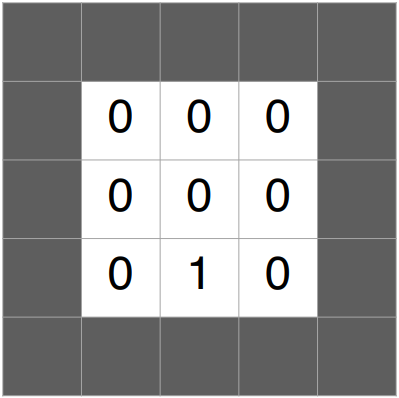
\includegraphics[width=0.35\linewidth]{pictures/binary_gridworld}}
    \caption[Coloring Environment]{Representations of the coloring environment}
    \label{fig:multipic_env} %% label for entire figure
\end{figure}

In the visualization \ref{fig:env} the outer dark cells show walls and the white cells are floors. The agent is represented with the red dot and the cell on which it is located is marked with the same color. By moving on the available space the agent can color more cells.  Every environment cell holds information about the object type it represents, being either walls, floors or agents. Furthermore, each object class contains information about its current color, whether it is accessible for an agent and, in case of a floor tile, if it is colored. Figure \ref{fig:bin_env} shows a simplified environment observation an agent processes each time step.

Floor cells manage the coloration state in binary form, as displayed in \ref{fig:bin_env}, with a one signalizing that the cell is colored. The environment reacts to agent movements by coloring the cells they visit. The environment is successfully solved, once all fields are colored. Otherwise, agents loose by using up a limited amount of steps. If a cell is already in coloration state one and an agent walks over it again the bit is switched, and the cell is reset to zero, removing its color. Besides moving up, down, left and right an agent can also execute the action wait, to stay in place.

\subsection{Compositions}

When multiple agents are placed in the coloring environment together, there are several ways how they will behave towards each other. Depending on the setting, even the environment distinguishes how certain actions affect the state. Per default agents will try to work together, to reach the environment goal. Alternatively, they could work independently or even compete with each other.

Each agent has a different random color. Cells adopt the color of the agent that walks over it. The primary focus in cooperative agent compositions however, is only the binary state. The agents always receive the same reward, regardless of the colors on the grid. An extreme example here would be one agent that colors the whole environment on its own. Naturally, this would result in a high reward and for cooperation this means that all other agents would get the same amount. 

In a DR setting however, agents are able to estimate their contribution, in order to improve their actions. This implementation executes the default action wait to find $G(z_{-i})$, see equation \eqref{eq:dr}. By choosing wait as the default action, agents can learn what the environment outcome and general coloration percentage would be if they had not participated in the current step. It is important to note here, that DR settings are always an extension of the cooperation mode and are never used together with other compositions and markets.

% The opposite is the case in competitive scenarios. 
In mixed-motive settings the colors are of importance. Agents only gain rewards based on their individual contributions. Thus, the rewards are generated by looking up each percentage a color is present and assigning that value to the same colored agent as reward. For example if a red agent colored 60\% of the grid red the reward for that agent would be 0.60. 

In a fully competitive mixed-motive scenario the reward calculations stay the same, only disabling the bit switching for opponent colors. Therefore, agents can directly capture already colored cells when they walk over them. However, if the cell contains the same color as the agent that moved on it, it is reset instead. Therefore, taking over the cells of the opponents is beneficial, since it increases the presence of the own color, leading to a higher reward.

In comparison, the basic mixed-motive composition shows no advantages resetting colored opponent cells. Instead, cell resets are always punished with a small negative reward, regardless of the composition. Hence, it is not likely that the agents work against each other in mixed-motive compositions, yielding a neutral or independent behavior between agents.

\subsection{Observation}
The observations agents receive from the environment are always generated from their individual point of view, with them in the center. The observation only contains a restricted area around them, making the environment a partially observable MDP. In large environments this feature increases the difficulty.
%but at the same time reflects the reality. 
An example for an observation of an agent is shown in \ref{fig:agent_obs}. This observation depicts the internal state of the environment visualization of image \ref{fig:env}.

\begin{figure}[hpbt]
    \centering
    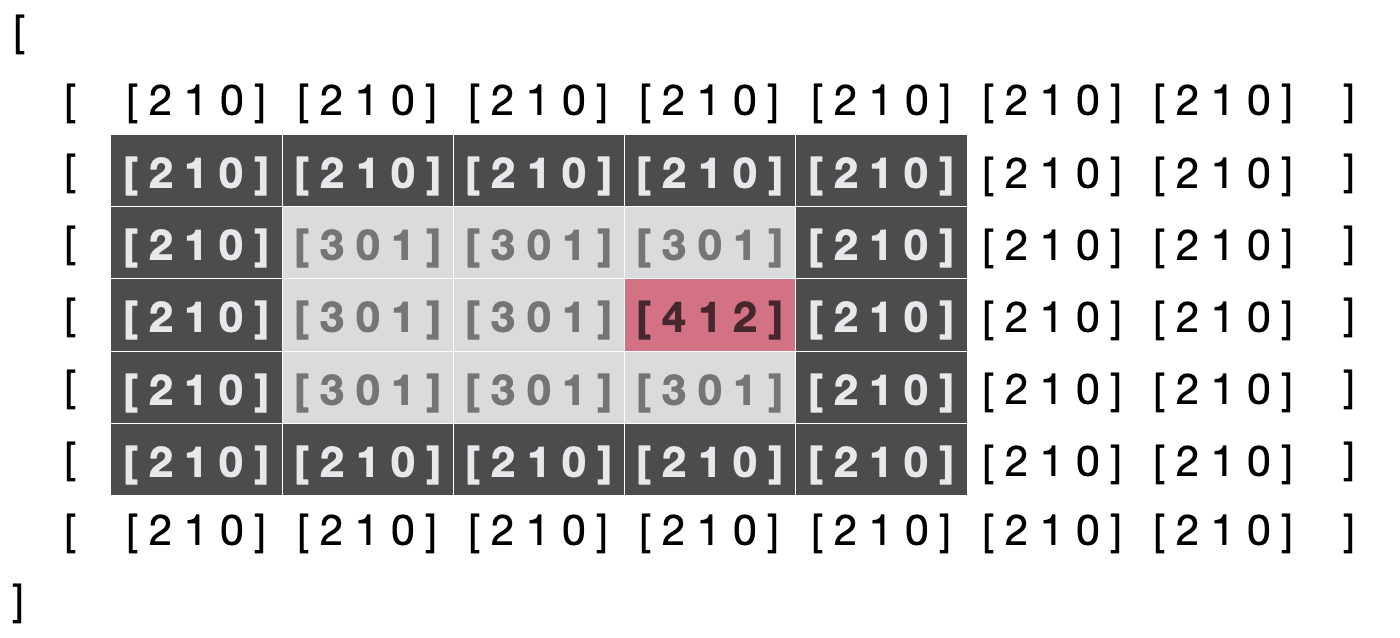
\includegraphics[width=0.8\textwidth]{pictures/agent_observation}\\
    \caption[Agent Observation]{The internal agent observation}\label{fig:agent_obs}
\end{figure}

Per default the agent has a view size of a seven by seven grid, represented in a three-dimensional array, similar to a picture with RGB information. Here, all highlighted entries are part of the grid that is shown in Figure \ref{fig:env} and the red array shows the agent. The first dimension of the observation array contains the whole internal observation of an agent. The second array dimension represents the environment grid. Since the view size of the agent exceeds the dimension of the 5x5 visual grid, the additional rows and columns are filled with placeholders, in this case walls. All highlighted row entries can be mapped to the columns of \ref{fig:env}, starting from the top left of the visualization. The last dimension contains cell information, which is always composed of three elements. 

% This also reduces the complexity of checking for a fully colored grid by just looking at all coloration states, regardless of the object type.

The first cell element defines the object type with one being just an empty cell, two shows a wall, three a floor tile and four an agent. The second element stores the coloration status, showing whether a cell is colored, with zero signalizing an uncolored cell. Since agents can not walk onto walls, represented as $[\;2\;1\;0\;]$, that object type always has a coloration state of one. The third cell encoding describes the color of a cell. To better distinguish the types in the visual representation, walls are zero for the color black and floors are initially white with encoding one. Each agent is assigned a number from two upwards which in turn stands for a randomly generated RGB color. The Floor color encoding is overwritten with the agents color code when the cell is captured. For example, should the agent move to the left, the cell of the previous position is now a colored Floor cell $[\;3\;1\;2\;]$. The new position of the agent is row three and column four with cell encoding $[\;4\;1\;2\;]$.

\section{Reward Calculations}\label{reward_calculations}
The allocation of rewards is closely related to the composition of the agents, which can be specified by the user in training or visualization runs. In addition, the environment shape can be set, a number of agents placed and more. A basic example command for a training run is shown in listing \ref{lst:command}.

\begin{lstlisting}[float=htp,caption=Exemplary command to execute training with three agents in a coloring environment using PPO as algorithm,label=lst:command,language=bash, numbers=left, numberstyle=\tiny, numbersep=8pt ,xleftmargin=3ex,xrightmargin=1ex]
$ python -m scripts.train
    --algo ppo
    --model ppo-training
    --env Empty-Grid-v0 
    --grid-size 7
    --agents 3 
    --max-steps 20
    --setting mixed-motive
\end{lstlisting}

The \verb|--algo| parameter can be either ``ppo'' or ``dqn'' to choose a learning algorithm. This argument is the only required setting for training. All other configurations, including those not listed in \ref{lst:command}, have default values and are shown in Appendix \ref{ax:training_params}.
%  discussed in the Sections \ref{learning_process} and \ref{market_settings}. An overview of all training parameters and their default values is listed in .
With \verb|--model| the destination path is defined, in which all logs, recordings and status updates are stored. Line 4 and 5 configures the environment. In alternative to the empty grid option of \verb|--env|, as shown in figure \ref{fig:env}, four homogeneous rooms can be generated with ``FourRooms-Grid-v0'' to increase the difficulty. The rooms are always of the same size and each room is accessible to all adjoining neighbors by one wall opening, which is random and changes in each episode. The overall size of the grid is set in Line 5. However, all grids in every layout option have outer walls that narrow the area in which agents can move. Hence, in a grid of size seven the agents can only move in a five by five field, due to the surrounding walls.

The amount of agents that act in the environment is set through the argument \verb|--agents| and the maximum quantity of steps they can execute is defined with \verb|--max-steps|. To gain the highest reward, the agents need to color the whole field before they run out of steps. Lastly, the argument \verb|--setting| specifies the composition of the agents. If no setting is set the agents work cooperatively. In the example of \ref{lst:command} the setting ``mixed-motive'' is chosen. The last two options here are ``mixed-motive-competitive'' and ``difference-reward''. % and ``percentage''.

Regardless of the composition, agents initially generate separate rewards in each step based on their individual environment change. For instance, agents that color a field produce a positive reward of 0.1, whereas agents that reset a field contribute a penalty of negative 0.1. Agents that just wait generate a reward of zero. The only exception is the setting ``mixed-motive-competitive'', since agents can capture opponent cells. If that is the case they get a positive reward of 0.1 otherwise the rules stay the same. 

Rewards are always written into a list, which is initially returned by the environment, see algorithm \ref{algo:step_reward}, line 1. The position in the list indicates the accountable agent, i.e. a reward list of $[0.1, 0, \cdots ]$ shows that agent zero is responsible for a reward of 0.1 and so forth. In algorithm \ref{algo:step_reward} the update process of the initial environment rewards during each step is summarized. This step function takes the training arguments of Appendix \ref{ax:training_params} into account, which leads to the four conditions below.

\begin{algorithm}[H]
    \DontPrintSemicolon
    observations, rewards, done, info = environment.step(actions)\;
    \;
    \uIf{difference reward setting} {
        rewards = calculate difference reward for each agent
    }
    \ElseIf{cooperative setting}{
        rewards = calculate one cooperative reward
    }
    \;
    \If{market specified}{
        rewards = execute market actions and return transaction rewards\;
    }
    \;
    \If{done}{
        rewards = calculate final rewards
    }
    \;
    \textbf{return} observations, rewards, done, info\;
    \caption{Reward calculation each step}\label{algo:step_reward}
\end{algorithm}

The first condition checks for a ``difference-reward'' setting. In this case, the agents work in cooperation but try to solve the CAP by calculating the DR, see function \eqref{eq:dr}. To achieve that, the current reward array is summed up, to summarize the overall reward. As a result the variable $G(z)$ of the DR equation is now set to the sum. To find the subtrahend of the equation, the agents are iterated, and their individual calculations take place. Here, the environment rewards are added up again, but this time the reward of the current agent is set to zero. This sum is the value of $G(z_{-i})$ for agent i. The function \eqref{eq:dr} is now applied for each agent and the initial reward list is updated with the individual DRs. 

The last step of the DR reward update is checking, whether any value exceeds an upper or lower bound. If that is the case then the value  is set to the corresponding limit. Otherwise, the reward stays as is. The upper and lower bounds are necessary, due to more participating agents possibly leading to a really big or very small sum. For example, very large sums without bounds could in turn decrease the importance of the final reward for reaching the environment goal. The other extreme are high negative sums demotivating agents to move. The bounds in this implementation are set to 0.1 and -0.1.

If the setting is set to the standard cooperation, the reward needs to be changed to a new homogeneous value for each agent, since they share the outcome. Again, the sum of the initial environment reward is calculated and reassigned to each agent position in the rewards array. The values must be clipped again in the same procedure as for the DR values. Here however, all rewards of the array are changed to the same clipped value, should the bounds be exceeded. Settings that contain ``mixed-motive'' skip all previous reward updates, since in this case each agent keeps their individual value.

As third condition the market argument is checked for a SM or AM. In this case the market transactions changes the rewards. Details of the market process are discussed in Section \ref{market_settings}. One thing to note here is, that agents can execute market transactions in each step. For example, they can spend their current reward on actions or shares that are for sale or receive the purchase price from buyers, which in turn modifies the rewards.

The last condition depends on the done flag which signalizes the end of an episode. The environment sets done to true, once either the grid is fully colored or the maximum step amount is reached. In this case, the final reward calculations are applied, see algorithm \ref{algo:final_reward}. The current rewards are passed as an argument to this calculation, since the list is modified again. %The result of those calculations is the final update of the reward variable.

\begin{algorithm}[H]
    \DontPrintSemicolon
    \eIf{mixed in setting}{
        \For(){each agent}{
            rewards[agent] += agent color percentage on the grid
        }
    }{// cooperative setting \;
        rewards += overall coloration percentage of the Grid
        
        \If {difference reward setting} {
            rewards = calculate difference rewards
        }
    }
    \;
    \If{market specified}{
        rewards = final market adjustments executed on rewards
    }
    \;
    \textbf{return} rewards\;
    \caption{Final reward calculation}\label{algo:final_reward}
\end{algorithm}

During the final reward calculations, the different agent compositions are checked again. In a ``mixed-motive'' or ``mixed-motive-competitive'' setting, each agents' grid coloration percentage, based on their color presence, is added to the individual reward. Otherwise, the composition is based on cooperation and the general grid coloration, regardless of the colors, is looked up and added to each reward value. 

Additionally, the presence of a DR setting needs to be checked here. For the final DR calculations the environment supplies information in the \verb|info| variable of algorithm \ref{algo:step_reward} Line 1. Namely, what the general coloration percentage of the environment would be for each agent, if this agent had executed action wait. Those percentages are subtracted from the cooperative coloration percentage to generate the DRs. Finally, the last market calculations are taken into account, see Chapter \ref{market_settings} for details.

\section{Learning Process}\label{learning_process}
In order to compare different settings and agent compositions easily, each agent manages its own learning improvement, observation and action selection. Therefore, all calculations and estimations are executed independently, for instance policy updates and value estimations. They also set up their own neural networks and optimizers and update them only with their own values. However, the environment still connects the agent experiences, by reacting to all agent actions simultaneously in each step and including visible agents in the observation.

Depending on the learning algorithm the corresponding class is instantiated by the training script, as shown in Figure \ref{fig:training}. The PPO and DQN classes both extend a base class that provides some abstract methods and a multiprocessing operation to execute actions on several environments at once. The base class returns data, allowing the training script to create recordings and log files to enable evaluation.

\begin{figure}[hpbt]
    \centering
    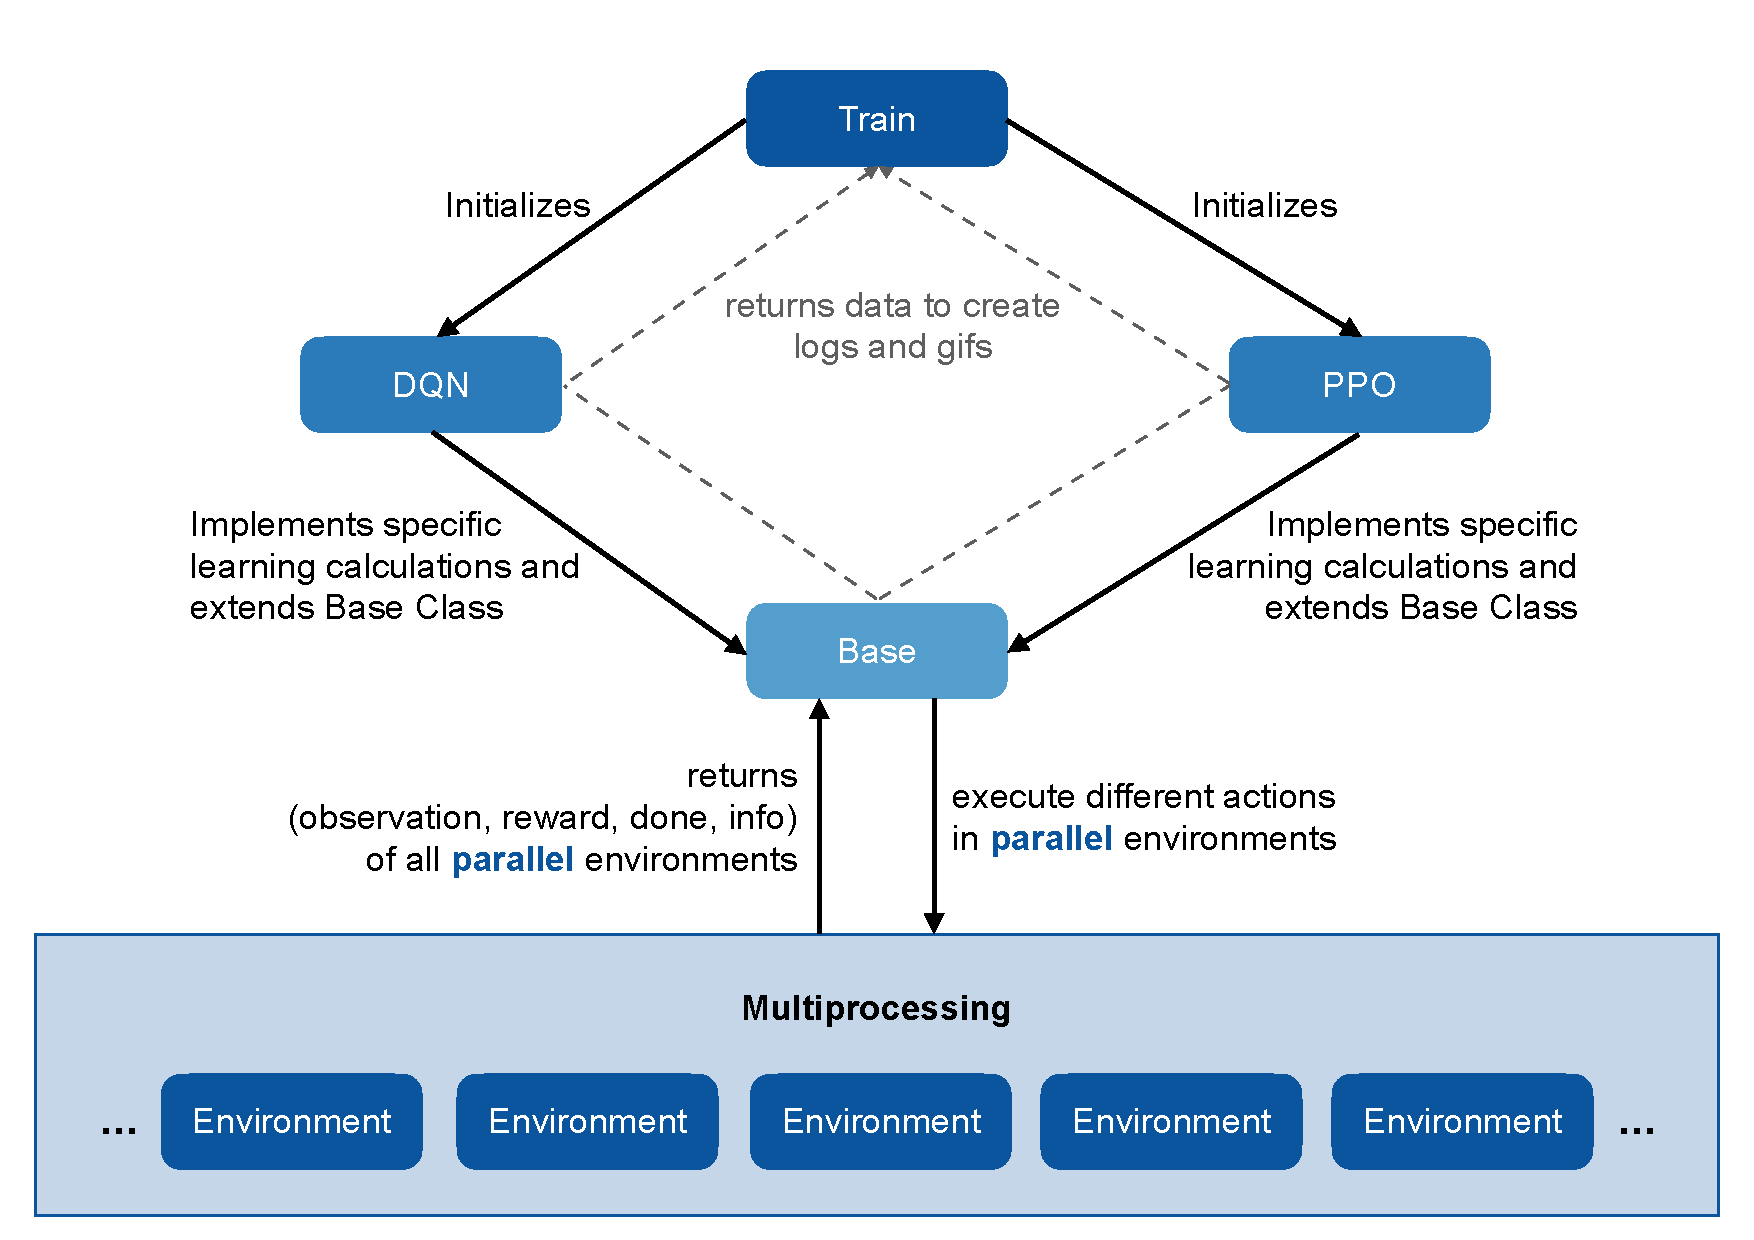
\includegraphics[width=0.9\textwidth]{pictures/training}\\
    \caption[The Training Structure]{The training structure}\label{fig:training}
\end{figure}

First, the training of agents begins by generating n environments based on the \verb|--procs| setting of the training command, see Appendix \ref{ax:training_params} for the parameter list. Each environment has the same configurations, for example \verb|--grid-size|, \verb|--agents| and \verb|--agent-view-size|. Second, the amount of \verb|--frames| is taken from the parameters, defining a general training loop, which ends once this number is reached or suceeded. During the loop, the defined training algorithm \verb|--algo| is executed.

Since both algorithms have similar procedures, they share the base class. In it a second iteration is triggered, that iterates over the amount set for \verb|--frames-per-procs|. During each step here, the agents execute actions in all parallel environments. Therefore, each step in the \verb|--frames-per-procs| iteration produces a frame in every environment. The action selection of the learning algorithms generate different decisions based on the state of each environment.

During the inner iteration, data like rewards, observations, actions and more are stored in base class variables that are accessible by the learning algorithms. When this iteration is done, the base variables are reset and log values of all episodes that reached the done state are returned to be logged, as shown in Figure \ref{fig:training}. The training loop keeps track of a frames counter, which sums up all frames that were produces by the parallel environments in the inner iteration. The training loop ends when the frames counter is greater or equal to \verb|--frames|. Otherwise, more experience batches are gathered.

Both learning algorithms include their own action selection methods. The PPO implementation relies on an actor-critic neural network, with an action space containing a probability distribution. In case of the DQN implementation the target network assigns Q values to actions, and agents choose one based on the maximum value with an epsilon greedy probability. In both variants the action selection results in one action for each agent and for each environment.

Unlike the PPO algorithm, in the DQN approach a quadruple of information is saved each frame into a replay memory. The four parts of the quadruple consist of the executed actions during that time step, the returned rewards and both the previous and new observation of the parallel environments. Until the frame amount of \verb|--initial-target-update| is reached, DQN agents only gather the quadruples but do not use them yet.

After exceeding the \verb|--initial-target-update|, the DQN learning starts. Each frame a batch of size \verb|--batch-size| is selected by randomly picking entries from the replay memory. Then, this batch is used to apply Q-learning updates to the experience samples, enhancing the training network. Every \verb|--target-update| amount of frames this training network is copied into the target network to enhance the action selection while keeping the algorithm stable.

The action selection itself is also improved during the training, by decreasing the $\epsilon$ gradually through $\epsilon = \epsilon_{end}+(\epsilon_{start}-\epsilon_{end})*e^{-\frac{frames}{decay}}$. This ensures exploration in the early phase. A high $\epsilon$ leads to actions that are picked at random. In the later course as the amount of frames increase, the $\epsilon$ gets smaller. In this case, the chance to select actions based on their Q values rises, which exploits the gathered experiences. Through \verb|--epsilon-start| and \verb|--epsilon-end| min and max values are set, and \verb|--epsilon-decay| defines the speed of reduction.

In the DQN implementation learning happens during the base class batch creation, whereas in the PPO algorithm the learning process is triggered after the creation of each base class experience batch. Basically, every time the inner loop finished, the gathered values are reshaped and saved into a PPO experience buffer. Additionally, the advantage values are calculated here and added to the buffer.

With that buffer the PPO model is now optimized. A small number of \verb|--epochs| are iterated and during each iteration random batch entries are selected. With those entries the entropies, values and losses are calculated. Afterwards, the calculation results are used to update the policy and network, as suggested in the code of \ref{fig:ppo_algo_code}.

\section{Market Settings}\label{market_settings}
To include a market into the training process, the \verb|--market| parameter can be set accordingly. The user has a choice to include an AM through the string ``am'' or a SM with ``sm''. In either case, the environment needs to adjust the action space, since agents now have the option to conduct market transactions.

Per default, the environment action space is discrete and only contains one element with five options: moving up, down, left, right or wait. Adding a market expands that discrete space into a multi discrete space. Hence, both markets require actions in form of arrays that contain three elements. However, they use different information in the action array slots. This and further distinctions and detailed procedures of each market are explained separately in the following.

\subsection{Shareholder Market}
A coloring environment that includes a SM constrains the first position of the action array to one of the five environment actions. The next position contains an agent index, towards which a buying offer will be made. Although, if this number is higher than the amount of agents in the game, the action intends no buying transaction. The last array position contains either a zero or a one, with one signalizing that the agent wants to sell its share. An abstract representation of a shareholder action array is: \verb|[environment_action, agent_index, sell_share]|.

\begin{figure}[hpbt]
    \centering
    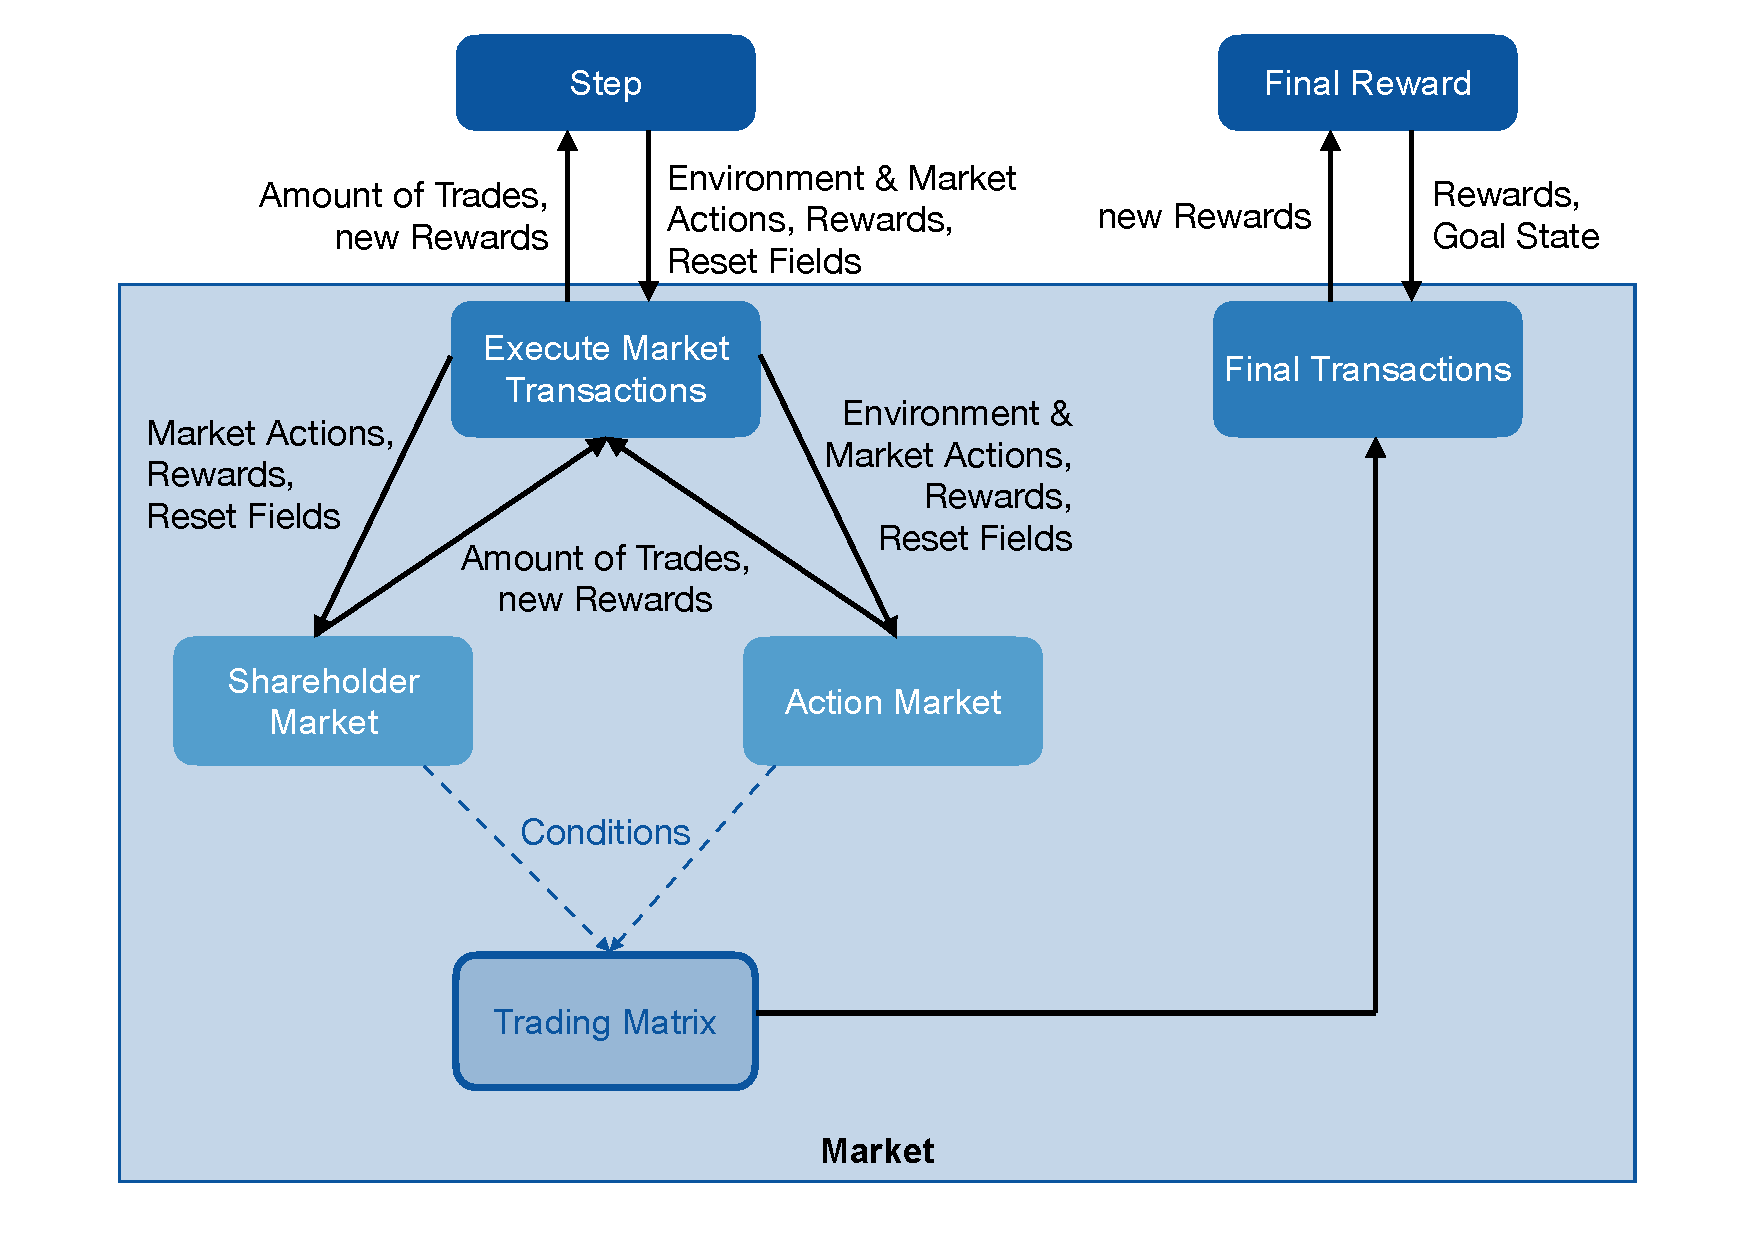
\includegraphics[width=0.9\textwidth]{pictures/market}\\
    \caption[Market Elements]{The market elements}\label{fig:market}
\end{figure}

In Figure \ref{fig:market} market elements are visualized. On the left, the process that takes place during each step is shown, see algorithm \ref{algo:step_reward} line 10. Here, the market always receives an action array that is already divided in two parts, one part only containing the first array position and the other part includes the buying and selling information in this case.
% Since transactions alter the rewards, the current reward is also transmitted. Lastly, an array of agent indices that have recently reset cells is also given, since some transaction conditions make use of that information.

In the course of the market calculations a trading matrix is altered. This matrix is quadratic with dimensions equal to the amount of agents. In a shareholder trading matrix, the diagonal contains ones, since every agent starts with the full ownership over their own shares. All other matrix slots are filled with zeros. An example for an initial trading matrix is shown below.
\begin{equation*}
trading\_matrix = 
\begin{pmatrix}
1 & 0 \\
0 & 1
\end{pmatrix}
\end{equation*}

The first thing to check in a market step execution is the market type. The type can be set with the \verb|--market| parameter and the market receives this setting during initialization. If the market type includes the string ``sm'' the SM matches and the corresponding function is called. 
% In this case the environment actions are not of importance, so the function receives all other parameters instead. 
Inside the shareholder function two additional matrices are created in each step, a buying matrix and a selling matrix. Both matrices are always initially filled with zeros, are quadratic, and their dimensions is equal to the amount of agents, similar to the trading matrix. Depending on the market action the buying matrix is altered to contain a one in the row of the buyer and the column of the agent that the offer is directed to.
% Here, the diagonal stays zero, since agents are prohibited of buying from themselves. 
Each agent can only buy one share at a time, therefore here the rows contain at maximum one entry. The same applies to the selling matrix, which contain ones on the diagonal for the agent that wants to sell according to the market actions.

After setting up and filling out the two matrices they are iterated, extracting the rows entries of each matrix and defining the corresponding indices as buyer and seller. A transaction takes place if the following conditions are met:
\begin{itemize}
    \item the buyer is not equal to the seller
    \item all entries of the buyer row and the seller row match
    \item the sellers shares are greater than the \verb|--trading-fee|
\end{itemize}

If all conditions are true, the trading matrix is updated here, by changing the share of the selling agent, adding the subtracted amount to the buyer. The amount can be set with \verb|--trading-fee|, which is 0.1 per default. The last condition ensures, that agents still receive some of their own rewards and do not trade everything off. 

An example for a transaction could be two agents acting in an environment. If agent two buys a share from agent one, the trading matrix is updated. The second row stores the shares of agent two, which increases by 0.1 on the first position. This signalizes that agent two is owner of some shares of agent one and still has 100\% of its own shares. In response, the shares in the first row and column of agent one decreases to 0.9.
\begin{equation*}
trading\_matrix = 
\begin{pmatrix}
1 & 0 \\
0 & 1
\end{pmatrix} \xrightarrow[\text{from Agent 1}]{\text{Agent 2 buys}} 
trading\_matrix = 
\begin{pmatrix}
0.9 & 0 \\
0.1 & 1
\end{pmatrix} 
\end{equation*}

Additionally, the rewards of the current step calculation, would be updated here, if a price for the shares are set. In this implementation however, the shares have no price since agents are willing to give them away for free. Otherwise, the price would be subtracted from the buying agents' reward and that value would be added to the reward of the selling agent. 

In any case, the SM triggers a reward calculation according to the trading matrix in every step. This means, that for the example above, agent two will receive 10\% of the rewards from agent one in every step, until the episode ends. However, this is only the case in the steps in which agent one is not in dept.

Further details of the reward calculations in markets will be discussed in Section \ref{market_reward_calc}. Lastly, the transaction count is documented for evaluation purposes. At this point the market execution for the current step is done and the number of executed trades and the updated rewards are returned to algorithm \ref{algo:step_reward}.

\subsection{Action Market}
The agent action shape of an AM environment is similar to the shareholder action array. Again, an action has three slots, with the first being the environment execution and the second being the index of an agent a buying offer is directed to. The difference to a shareholder action is the last array position. Instead of setting a bit here to signalize the willingness of selling shares, the agent chooses an environment action that is expected from the agent of position two. Hence, an abstract representation of an action in the AM is the following: \verb|[environment_action, agent_index, expected_action]|.

The market elements and general process of visualization \ref{fig:market} also apply to an AM setting. Here however, the trading matrix is initially filled with zeros. 
% Furthermore, the AM function needs all parameters, including the environment actions. This information is crucial to the transaction conditions, which are:
To establish a transaction the market actions are examined, and the following conditions checked:
\begin{itemize}
    \item the buyer differs from the receiving agent
    \item the environment action of the receiving agent matches the expected action
\end{itemize}

When the two conditions apply a market transaction takes place. The \verb|--trading-fee| parameter decides the price the buyer pays the receiving agent. Both the rewards and trading matrix are altered here, by subtracting the price from the buyer and adding it to the receiver. An example of the trading matrix update in this market setup is shown below. Here again agent two is purchasing from agent one.
\begin{equation*}
trading\_matrix = 
\begin{pmatrix}
0 & 0 \\
0 & 0
\end{pmatrix} \xrightarrow[\text{from Agent 1}]{\text{Agent 2 buys}} 
trading\_matrix = 
\begin{pmatrix}
0 & 0.1 \\
0 & -0.1
\end{pmatrix} 
\end{equation*}

The trading matrix stores the market balance of both agents in each row. For agent two this means that the negative value was spent. The first row shows that agent one still has a neutral balance and gained the \verb|--trading-fee| of 0.1 from agent two. To conclude, the market returns the number of transactions that took place in this step and the new rewards.

\subsection{Reward Calculations}\label{market_reward_calc}
During each step agents can update the trading matrix by acting on the market. With each update the rewards are also changed. In Figure \ref{fig:market_rewards} a detailed example of the reward update in a market is shown. It is worth mentioning that it is not possible to execute both markets simultaneously, but rather one or none must be set for a training process. This illustration shows both calculations in one image for convenience. Equal to the previous examples, the red agent two buys a share or action from the blue agent one. For both market scenarios the \verb|--trading-fee| is set to the default value and both agent rewards start at 0.1. On the top half of the image the internal market calculation of a SM is shown, and the bottom half illustrates the calculation of an AM.
\begin{figure}[hpbt]
    \centering
    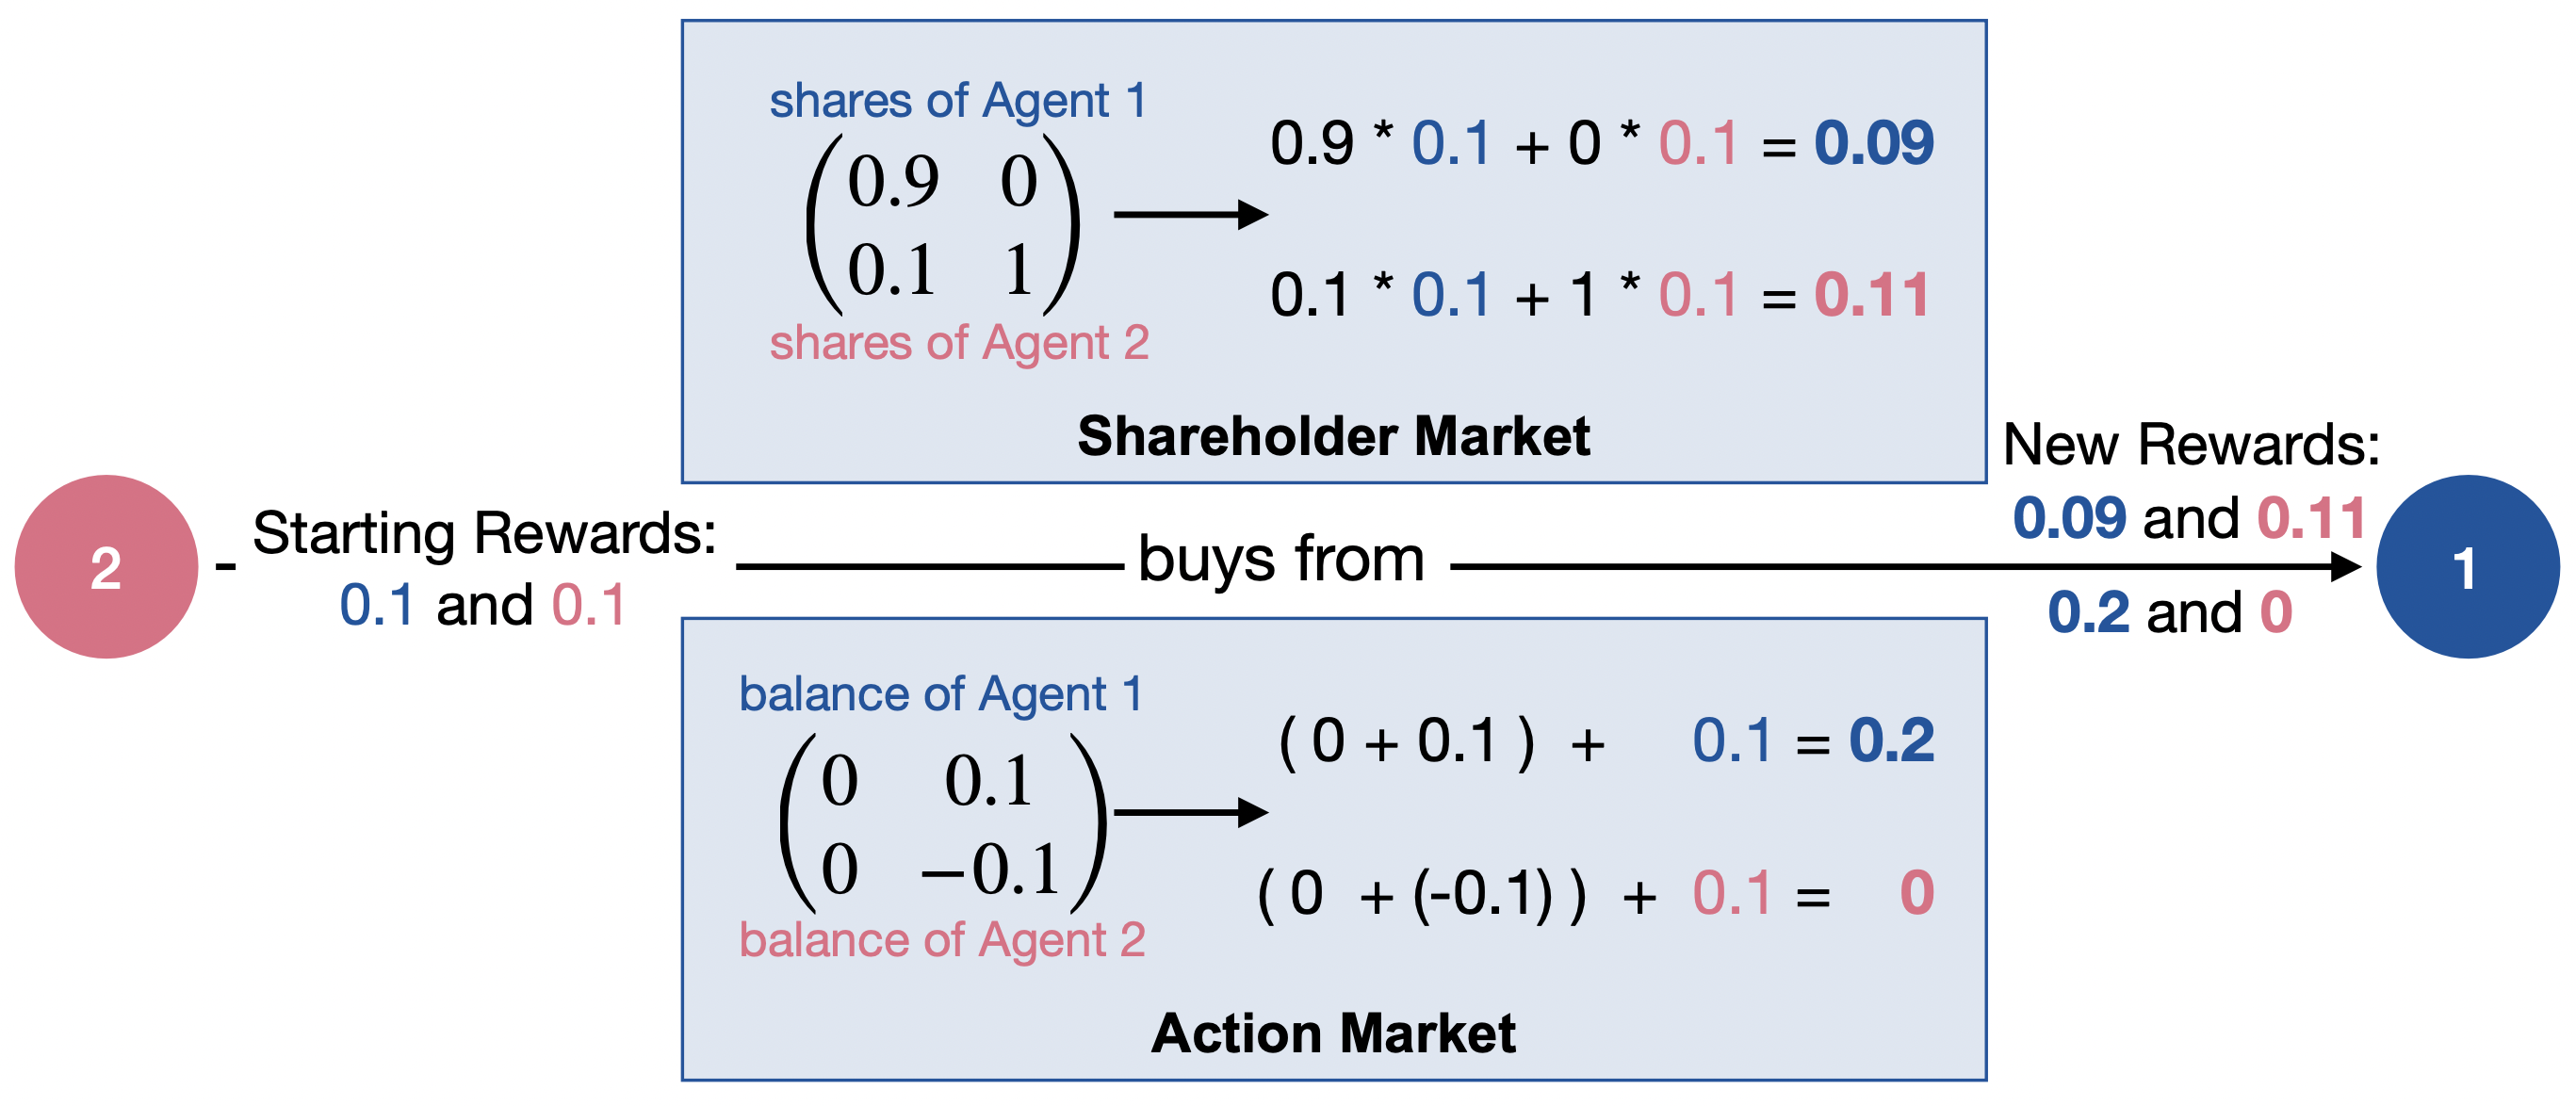
\includegraphics[width=0.9\textwidth]{pictures/new_market_rewards}\\
    \caption[Exemplary Reward Calculation Of Markets]{Exemplary reward calculations of both market types}\label{fig:market_rewards}
\end{figure}

In a SM the trading matrix represents the distribution of agent shares. Each matrix column adds up to one, representing a 100\% share of an agent. As mentioned earlier the diagonal of the matrix is initially set to one since agents start with complete ownership over their shares. For this example the trading matrices are configured accordingly. The first matrix row implies that agent one is owner of 90\% of its own shares and is not owner of any shares from agent two. Whereas the second row shows that agent two claims 10\% of the shares of agent one and has full ownership over its own.

To generate the new rewards of the agents, the market multiplies all current rewards with each matrix rows. The resulting products of each row are then summed up to represent the new reward of the corresponding agent. For the example, agent one gets a new reward value of 0.09 and agent two claims 0.01 from agent one and adds that to its full value of 0.1, resulting in a new reward of 0.11. 

In contrast to an AM in a SM the rewards are just reassigned based on the current shares of the trading matrix. An exception occurs, when agents have negative rewards. In this case their share will be skipped during the redistribution, since shares are used to participate in profits. 

Another difference to AMs is that the shown SM reward redistributions are executed in each step, and it is irrelevant whether market actions were executed. The only exception however is the last step, when the done flag is set to true. In this case the final rewards, see algorithm \ref{algo:final_reward}, need to be calculated first, before the shares are taken into account.

AMs, in most cases, update the rewards directly and only once, when a transaction is executed. The trading fee is immediately subtracted from one agents' reward and added to the counterpart during the trade. If an agent can not afford the fee the process is completed anyway and the agent goes into debt. 

Thus, this market type makes no use of the trading matrix. Nonetheless, the matrix is always updated, since a specific scenario requires the calculations to be executed at the end, see Section \ref{market_conditions}. In this case, the agents market balance, stored in the matrix rows, is summed up and added to the current reward. This procedure is illustrated in the bottom half of figure \ref{market_reward_calc}. Here, the fee of 0.1 is subtracted from agent two and added to the reward of agent one, leading to new rewards of 0.2 for agent one and zero for agent two.

\subsection{Additional Conditions}\label{market_conditions}
The \verb|--market| string for both types can be extended to add more conditions, namely with ``no-reset'', ``no-debt'' and ``goal''. The ``no-reset'' string enables the check whether the buyer has recently reset a cell. If that is the case, the corresponding buyers are ignored on the market for the current step. Hence, their market actions will not be applied. However, in a SM the penalized agent can still sell its shares. 

With the ``no-debt'' Flag, transactions only take place if buyers can afford to pay the price. In this implementation with AMs and the default fee, this is solely the case if agents have colored a cell in that step. Waiting or misbehaving agents are excluded as buyers, since their rewards result in 0 or -0.1, which does not meet the fee of 0.1. For SMs this depends on the presence of a share price. Per default the price is zero, similar to the approach of Schmid et al. \cite{scbe21}, making this condition irrelevant for the SM setting.
% TODO kommt zu goal Both market conditions can be used simultaneously.

The last addition, ``goal'', lets the market process run as usual, only removing the reward changes during the steps. Here, all transactions are just documented into the trading matrix during an episode. Eventually, the transactions are executed once the final rewards of algorithm \ref{algo:final_reward} is calculated. As shown on the right side of Figure \ref{fig:market}, the market obtains those rewards and a Boolean describing whether the environment goal was reached.

The rewards are updated with the trading matrix content when either of the two conditions is satisfied:
\begin{itemize}
    \item ``goal'' addition is present and environment goal was reached
    \item no ``goal'' addition and market type is a SM
\end{itemize}
Otherwise the rewards are return as they are and will not be processed further. 

For such goal oriented markets, regardless of the type, the final environment state needs to equal the overall aim. Thus, the whole grid has to be colored, to execute the final market transactions.

% Since the goods of a SM are shares, naturally the current reward values are of importance. During the step calculations of the rewards the done flag is  takes place at the end of an episode. In an AM however, each step is self-contained in regards to transactions and payouts. Nonetheless, with the ``goal'' addition, the payout also shifts to the end of episodes. 

If the first condition applies and an AM is present the rewards are updated by using the trading matrix. For a SM either condition must be met in order to generate the final reward. The calculations for both cases are equal to the example of Chapter \ref{market_reward_calc}.
% Again, the trading matrix rows and rewards are iterated here. Each row element is multiplied with the reward of the same index and added to the new reward of that agent. An example of both operations is shown in Figure \ref{fig:market_rewards}.

After the final market updates to the rewards the new values are returned, as shown in Figure \ref{fig:market}. The last thing to point out is that the additional market conditions can be used in combination, making ``sm-goal-no-reset-no-debt'' for example a valid \verb|--market| setting.